\documentclass{article}

\usepackage[T1]{fontenc}
\usepackage{textcomp}

\usepackage[english]{babel}
\usepackage[utf8]{inputenc}

\usepackage{lmodern}

\usepackage{hyperref}
\hypersetup{breaklinks}
\hypersetup{pdfborder=0 0 0}

\usepackage[babel=true]{microtype}

\usepackage{amsmath}

\usepackage{geometry}

\usepackage{tikz}

\usepackage[normalem]{ulem}


\title{The impact of vector interaction with other insect species on
  disease spread}

\author{
  Elizabeth Borer
  \and
  David Crowder
  \and
  Deborah Finke
  \and
  Jing Li
  \and
  Jan Medlock
  \and
  David Pattemore
  \and
  Rakefet Sharon
}


\newcommand{\md}{\mathrm{d}}
\newcommand{\me}{\mathrm{e}}
\newcommand{\mat}[1]{\mathbf{#1}}
\renewcommand{\vec}[1]{\mathbf{#1}}

\newcommand{\comment}[1]{\textbf{#1}}


\begin{document}

\maketitle

\section{Model}

Let $V_{sm}(t)$ and $V_{im}(t)$ be the number of susceptible and
infectious vectors moving at time $t$, $V_{sfs}(t)$ and $V_{ifs}(t)$
be the number of susceptible and infectious vectors feeding on
susceptible plants at time $t$, and $V_{sfi}(t)$ and $V_{ifi}(t)$ be
the number of susceptible and infectious vectors feeding on infectious
plants at time $t$.  Likewise, let $P_s(t)$ and $P_i(t)$ be the number
of susceptible and infected plants at time $t$.  The total number of vectors is
\begin{equation}
  V = V_{sm} + V_{im} + V_{sfs} + V_{ifs} + V_{sfi} + V_{ifi}
\end{equation}
and the total number of plants is
\begin{equation}
  P = P_s + P_i.
\end{equation}
The vectors feed on new plants at the rate $f_V$ and spend the
proportion $\phi_V$ of their time feeding and $1 - \phi_V$ moving.  We
assume that vectors only reproduce when they are feeding; the birth
rate is proportional to the number of the feeding vectors, with a
logistic term dependent on the total number of vectors; and the
newborns join the moving group.  Moving and feeding vectors die but at
different rates, with moving vectors assumed to die more quickly than
feeding vectors (i.e.~$\delta_V > 0$).

The model is
\begin{equation}
  \label{odesystem}
  \begin{split}
    \frac{\md V_{sm}}{\md t}
    &=
    - \underbrace{\frac{f_V}{1 - \phi_V} V_{sm}}_{\text{to feeding}}
    + \underbrace{\frac{f_V}{\phi_V} (V_{sfs} + V_{sfi})}_{\text{from feeding}}
    + \underbrace{\gamma_V V_{im}}_{\text{loses pathogen}}
    - \underbrace{(1 + \delta_V) \mu_V V_{sm}}_{\text{death}}
    \\ & \quad\quad {}
    + \underbrace{b_V V_f \left(1 - \frac{V}{K_V P}\right)}_{\text{birth}},
    \\
    \frac{\md V_{sfs}}{\md t}
    &=
    \underbrace{\frac{f_V}{1 - \phi_V} \frac{P_s}{P} V_{sm}}_{\text{from moving}}
    - \underbrace{\frac{f_V}{\phi_V} V_{sfs}}_{\text{to moving}}
    + \underbrace{\gamma_V V_{ifs}}_{\text{loses pathogen}}
    - \underbrace{\mu_V V_{sfs}}_{\text{death}}
    - \underbrace{\beta_P \frac{V_{ifs}}{P_s} V_{sfs}}_{\text{plant
        infected}}
    + \underbrace{\gamma_P V_{sfi}}_{\text{plant clears pathogen}},
    \\
    \frac{\md V_{sfi}}{\md t}
    &=
    \underbrace{\frac{f_V}{1 - \phi_V} \frac{P_i}{P} V_{sm}}_{\text{from moving}}
    - \underbrace{\frac{f_V}{\phi_V} V_{sfi}}_{\text{to moving}}
    + \underbrace{\gamma_V V_{ifi}}_{\text{loses pathogen}}
    - \underbrace{\mu_V V_{sfi}}_{\text{death}}
    + \underbrace{\beta_P \frac{V_{ifs}}{P_s} V_{sfs}}_{\text{plant infected}}
    - \underbrace{\gamma_P V_{sfi}}_{\text{plant clears pathogen}}
    \\ & \quad\quad {}
    - \underbrace{\beta_V V_{sfi}}_{\text{infection}},
    \\
    \frac{\md V_{im}}{\md t}
    &=
    - \underbrace{\frac{f_V}{1 - \phi_V} V_{im}}_{\text{to feeding}}
    + \underbrace{\frac{f_V}{\phi_V} (V_{ifs} + V_{ifi})}_{\text{from feeding}}
    - \underbrace{\gamma_V V_{im}}_{\text{loses pathogen}}
    - \underbrace{(1 + \delta_V) \mu_V V_{im}}_{\text{death}},
    \\
    \frac{\md V_{ifs}}{\md t}
    &=
    \underbrace{\frac{f_V}{1 - \phi_V} \frac{P_s}{P} V_{im}}_{\text{from moving}}
    - \underbrace{\frac{f_V}{\phi_V} V_{ifs}}_{\text{to moving}}
    - \underbrace{\gamma_V V_{ifs}}_{\text{loses pathogen}}
    - \underbrace{\mu_V V_{ifs}}_{\text{death}}
    - \underbrace{\beta_P \frac{V_{ifs}}{P_s} V_{ifs}}_{\text{plant infected}}
    + \underbrace{\gamma_P V_{ifi}}_{\text{plant clears pathogen}},
    \\
    \frac{\md V_{ifi}}{\md t}
    &=
    \underbrace{\frac{f_V}{1 - \phi_V} \frac{P_i}{P} V_{im}}_{\text{from moving}}
    - \underbrace{\frac{f_V}{\phi_V} V_{ifi}}_{\text{to moving}}
    - \underbrace{\gamma_V V_{ifi}}_{\text{loses pathogen}}
    - \underbrace{\mu_V V_{ifi}}_{\text{death}}
    + \underbrace{\beta_P \frac{V_{ifs}}{P_s} V_{ifs}}_{\text{plant infected}}
    - \underbrace{\gamma_P V_{ifi}}_{\text{plant clears pathogen}}
    \\ & \quad\quad {}
    + \underbrace{\beta_V V_{sfi}}_{\text{infection}},
    \\
    \frac{\md P_s}{\md t}
    &=
    - \underbrace{\beta_P V_{ifs}}_{\text{infection}}
    + \underbrace{\gamma_P P_i}_{\text{clears pathogen}},
    \\
    \frac{\md P_i}{\md t}
    &=
    \underbrace{\beta_P V_{ifs}}_{\text{infection}}
    - \underbrace{\gamma_P P_i}_{\text{clears pathogen}},
  \end{split}
\end{equation}
where the number of feeding vectors is
$V_f = V_{sfs} + V_{sfi} + V_{ifs} + V_{ifi}$, $\beta_V$ is the
infection rate from plants to vectors, $\beta_P$ is the infection rate
from vectors to plants, $\gamma_V$ is the rate of pathogen clearance
in vectors, $\mu_V$ is the death rate of the feeding vectors,
$\delta_V$ is the proportional increase in the death rate for moving
vectors, $b_V$ is the birth rate of vectors, and $K_V$ is the carrying
capacity of vectors per plant (\autoref{fig:full_model_diagram}).

\begin{figure}
  \centering
  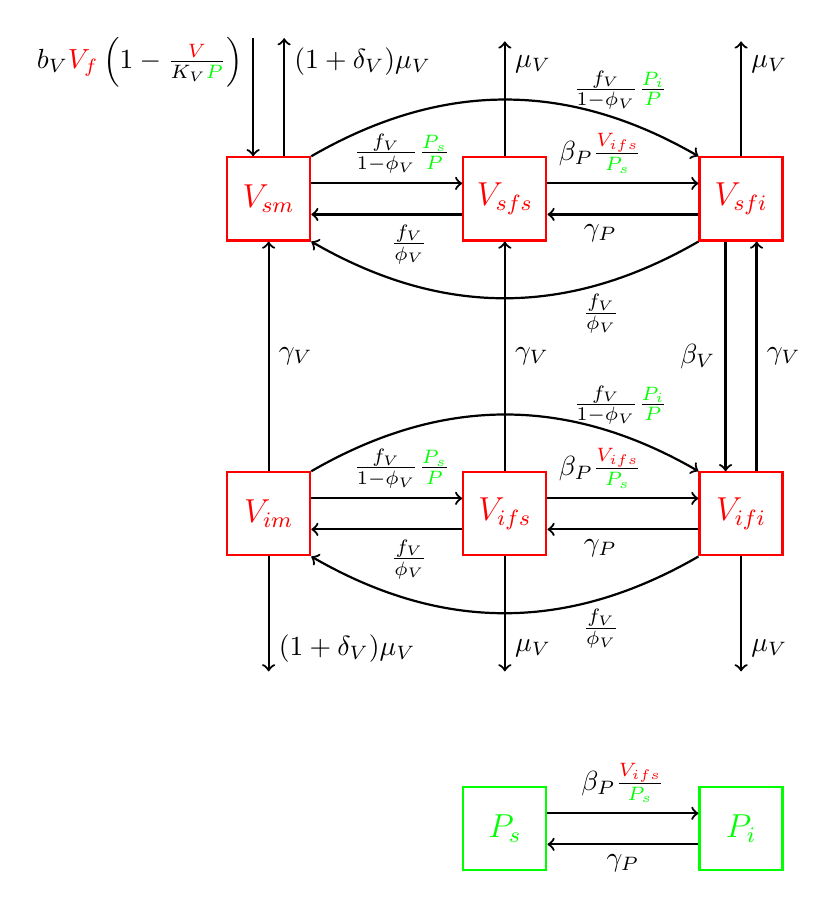
\begin{tikzpicture}[
    thick,
    scale = 1,
    compartment/.style = {draw,
      font = \large,
      minimum size = {3em}},
    plant/.style = {green},
    vector/.style = {red},
    ]

    \node at (0, 8)
    [compartment, vector, name = V_sm] {$V_{sm}$};
    \node at (0, 4)
    [compartment, vector, name = V_im] {$V_{im}$};

    \node at (3, 8)
    [compartment, vector, name = V_sfs] {$V_{sfs}$};
    \node at (3, 4)
    [compartment, vector, name = V_ifs] {$V_{ifs}$};

    \node at (6, 8)
    [compartment, vector, name = V_sfi] {$V_{sfi}$};
    \node at (6, 4)
    [compartment, vector, name = V_ifi] {$V_{ifi}$};

    \node at (3, 0)
    [compartment, plant, name = P_s] {$P_s$};
    \node at (6, 0)
    [compartment, plant, name = P_i] {$P_i$};

    \draw [->] (P_s.20) to node [above]
    {$\beta_P \frac{\textcolor{red}{V_{ifs}}}{\textcolor{green}{P_s}}$}
    (P_i.160);

    \draw [->] (P_i.200) to node [below] {$\gamma_P$} (P_s.340);

    \draw [->] (V_sfi.250) to node [left] {$\beta_V$} (V_ifi.110);

    \draw [->] (V_im) to node [right] {$\gamma_V$} (V_sm);
    \draw [->] (V_ifs) to node [right] {$\gamma_V$} (V_sfs);
    \draw [->] (V_ifi.70) to node [right] {$\gamma_V$} (V_sfi.290);

    \draw [->] (V_sm.20) to node [above, pos = 0.6]
    {$\frac{f_V}{1 - \phi_V}
      \frac{\textcolor{green}{P_s}}{\textcolor{green}{P}}$}
    (V_sfs.160);
    \draw [->] (V_sm.45) to [bend left = 30] node [above, pos = 0.8]
    {$\frac{f_V}{1 - \phi_V}
      \frac{\textcolor{green}{P_i}}{\textcolor{green}{P}}$}
    (V_sfi.135);

    \draw [->] (V_im.20) to node [above, pos = 0.6]
    {$\frac{f_V}{1 - \phi_V}
      \frac{\textcolor{green}{P_s}}{\textcolor{green}{P}}$}
    (V_ifs.160);
    \draw [->] (V_im.45) to [bend left = 30] node [above, pos = 0.8]
    {$\frac{f_V}{1 - \phi_V}
      \frac{\textcolor{green}{P_i}}{\textcolor{green}{P}}$}
    (V_ifi.135);

    \draw [->] (V_sfs.200) to node [below, pos = 0.35]
    {$\frac{f_V}{\phi_V}$} (V_sm.340);
    \draw [->] (V_sfi.225) to [bend left = 30] node [below, pos = 0.25]
    {$\frac{f_V}{\phi_V}$} (V_sm.315);

    \draw [->] (V_ifs.200) to node [below, pos = 0.35]
    {$\frac{f_V}{\phi_V}$} (V_im.340);
    \draw [->] (V_ifi.225) to [bend left = 30] node [below, pos = 0.25]
    {$\frac{f_V}{\phi_V}$} (V_im.315);

    \draw [->] (V_sfs.20) to node [above, pos = 0.35]
    {$\beta_P \frac{\textcolor{red}{V_{ifs}}}{\textcolor{green}{P_s}}$}
    (V_sfi.160);
    \draw [->] (V_ifs.20) to node [above, pos = 0.35]
    {$\beta_P \frac{\textcolor{red}{V_{ifs}}}{\textcolor{green}{P_s}}$}
    (V_ifi.160);

    \draw [->] (V_sfi.200) to node [below, pos = 0.65]
    {$\gamma_P$} (V_sfs.340);
    \draw [->] (V_ifi.200) to node [below, pos = 0.65]
    {$\gamma_P$} (V_ifs.340);

    \draw [<-] (V_sm.110) to node [left, pos = 0.8]
    {$b_V \textcolor{red}{V_f}
      \left(1 - \frac{\textcolor{red}{V}}{K_V \textcolor{green}{P}}\right)$}
    +(90: 1.5);

    \draw [->] (V_sm.70) to node [right, pos = 0.8]
    {$(1 + \delta_V) \mu_V$} +(90: 1.5);
    \draw [->] (V_im) to node [right, pos = 0.8]
    {$(1 + \delta_V) \mu_V$} +(270: 2);

    \draw [->] (V_sfs) to node [right, pos = 0.8]
    {$\mu_V$} +(90: 2);
    \draw [->] (V_ifs) to node [right, pos = 0.8]
    {$\mu_V$} +(270: 2);

    \draw [->] (V_sfi) to node [right, pos = 0.8]
    {$\mu_V$} +(90: 2);
    \draw [->] (V_ifi) to node [right, pos = 0.8]
    {$\mu_V$} +(270: 2);

  \end{tikzpicture}
  \caption{Model diagram.  $P_s$ and $P_i$ (green) are the numbers
    of uninfected and plants.  $V_{sm}$ and $V_{im}$ are the numbers
    of susceptible and infectious vectors moving, $V_{sfs}$ and
    $V_{ifs}$ are numbers of susceptible and infectious vectors
    feeding on susceptible plants, and $V_{sfi}$ and $V_{ifi}$ are the
    numbers of susceptible and infectious vectors feeding on
    infectious plants.}
  \label{fig:full_model_diagram}
\end{figure}


\begin{table}
  \centering
  \begin{tabular}{llr}
    \multicolumn{2}{l}{\textbf{Parameter}}
    & \multicolumn{1}{r}{\textbf{Value}}
    \\
    $f_V$ & Plants fed on per unit time & $6\;\text{d}^{-1}$
    \\
    $\phi_V$ & Fraction of time vectors spend feeding & $0.5$
    \\
    $\mu_V$ & Mortality rate for feeding vectors & $0.02\;\text{d}^{-1}$
    \\
    $\delta_V$ & Relative mortality increase for moving vectors & $1$
    \\
    $b_V$ & Fecundity of feeding vectors & $0.08\;\text{d}^{-1}$
    \\
    $K_V$ & Carrying capacity of vectors per plant & $100$
    \\
    $\gamma_P$ & Rate of pathogen clearance in plants & $0\;\text{d}^{-1}$
    \\
    $V(0)$ & Initial number of vectors & $100$
    \\
    $P(0)$ & Initial number of susceptible & $10\,000$
    \\
    \multicolumn{3}{c}{\textbf{Persistent}}
    \\
    $\beta_V$ & Transmission rate from plants to vectors & $0.48\;\text{d}^{-1}$
    \\
    $\beta_P$ & Transmission rate from vectors to plants & $0.48\;\text{d}^{-1}$
    \\
    $\gamma_V$ & Rate of pathogen clearance in vectors & $0\;\text{d}^{-1}$
    \\
    \multicolumn{3}{c}{\textbf{Non-persistent}}
    \\
    $\beta_V$ & Transmission rate from plants to vectors & $4.8\;\text{d}^{-1}$
    \\
    $\beta_P$ & Transmission rate from vectors to plants & $4.8\;\text{d}^{-1}$
    \\
    $\gamma_V$ & Rate of pathogen clearance in vectors & $0.12\;\text{d}^{-1}$
  \end{tabular}
  \caption{Model parameters and initial conditions.}
  \label{params}
\end{table}


\section{Results}

\begin{itemize}
\item The pathogen grows slowly until the vector population becomes
  large (\autoref{fig:solutions}).

\item The pathogen growth rate increases as the vector population
  grows (\autoref{fig:growth_rates}).

\item The growth rate is insensitive to the feeding rate
  (\hyperref[fig:sensitivity_1param]{Figures
    \ref*{fig:sensitivity_1param}}--\ref{fig:sensitivity_2params}).
\end{itemize}


\begin{figure}
  \centering
  \includegraphics[width = \textwidth]{solutions_new}
  \caption{Model solutions for persistent and non-persistent
    scenarios.  Parameter values are given in \autoref{params}.
    For initial conditions, we used the result from the quasi-steady
    state approximation (\autoref{sec:QSSA}) that $50\%$ of the
    vectors are moving and $50\%$ are feeding for our parameter
    values, and that 1 of the moving vectors are infected and all
    others are uninfected ($V_{sm}(0) = 49, V_{im}(0) = 1, V_{sfs}(0) =
    50, V_{sfi}(0) = V_{ifs}(0) = V_{ifi}(0) = 0$).}
  \label{fig:solutions}
\end{figure}

\begin{figure}
  \centering
  \includegraphics[width = \textwidth]{growth_rates_new}
  \caption{Intrinsic growth rate of the pathogen.  Model initial
    conditions were the disease-free state given by the parameters
    (\autoref{params}) and the result from the quasi-steady state
    approximation (\autoref{sec:QSSA}) that $50\%$ of the vectors are
    moving and $50\%$ are feeding for our parameter values ($V_{sm}(0)
    = V_{sfs}(0) = 50, P_s(0) = 10\,000, V_{im}(0) = V_{sfi}(0) =
    V_{ifs}(0) = V_{ifi}(0) = P_i(0) = 0$).}
  \label{fig:growth_rates}
\end{figure}

\begin{figure}
  \centering
  \includegraphics[width = \textwidth]{sensitivity_1param_new}
  \caption{Intrinsic growth rate of the pathogen vs.~parameter values
    at $150~\text{d}$, relative to its value for the baseline
    parameter value.  The dotted horizontal lines show the baseline
    parameter values.  Parameter values and initial conditions are as
    in \autoref{fig:growth_rates}.}
  \label{fig:sensitivity_1param}
\end{figure}

\begin{figure}
  \centering
  \includegraphics[width = \textwidth]{sensitivity_1param_new_fV}
  \caption{Intrinsic growth rate of the pathogen vs.~the feeding rate
    ($f_V$) at $150~\text{d}$, relative to its value for the baseline
    parameter value.  The vertical axis has a linear scale, compared
    to a log scale in \autoref{fig:growth_rates}, to show the smaller
    differences in growth rate as feeding rate varies.  The dotted
    horizontal lines show the baseline parameter values.  Parameter
    values and initial conditions are as in
    \autoref{fig:growth_rates}.}
  \label{fig:sensitivity_1param_fV}
\end{figure}

\begin{figure}
  \centering
  \includegraphics[width = \textwidth]{sensitivity_2params_new}
  \caption{Intrinsic growth rate of the pathogen vs.~parameter values
    at $150~\text{d}$, relative to its value for the baseline
    parameter value.  Parameter values and
    initial conditions are as in \autoref{fig:growth_rates}.}
  \label{fig:sensitivity_2params}
\end{figure}


\clearpage
\appendix
\section{Quasi-steady-state approximation}
\label{sec:QSSA}

Under the quasi-steady-state approximation, we take the movement rate
to be fast relative to all the other rates, i.e.~$f_V \to \infty$ and
all other parameters $\operatorname{O}(1)$.  Then terms in $f_V$ from
the differential equations give
\begin{equation}
  \begin{split}
    \frac{1}{1 - \phi_V} V_{sm} &= \frac{1}{\phi_V} (V_{sfs} + V_{sfi}),
    \\
    \frac{1}{1 - \phi_V} \frac{P_s}{P} V_{sm} &= \frac{1}{\phi_V} V_{sfs},
    \\
    \frac{1}{1 - \phi_V} \frac{P_i}{P} V_{sm} &= \frac{1}{\phi_V} V_{sfi},
    \\
    \frac{1}{1 - \phi_V} V_{im} &= \frac{1}{\phi_V} (V_{ifs} + V_{ifi}),
    \\
    \frac{1}{1 - \phi_V} \frac{P_s}{P} V_{im} &= \frac{1}{\phi_V} V_{ifs},
    \\
    \frac{1}{1 - \phi_V} \frac{P_i}{P} V_{im} &= \frac{f_V}{\phi_V} V_{ifi}.
  \end{split}
\end{equation}
Thus, the QSSA is
\begin{equation}
  \begin{aligned}
    V_{sm} &= (1 - \phi_V) V_s,
    &
    V_{sfs} &= \phi_V \frac{P_s}{P} V_s,
    &
    V_{sfi} &= \phi_V \frac{P_i}{P} V_s,
    \\
    V_{im} &= (1 - \phi_V) V_i,
    &
    V_{ifs} &= \phi_V \frac{P_s}{P} V_i,
    &
    V_{ifi} &= \phi_V \frac{P_i}{P} V_i,
  \end{aligned}
\end{equation}
with
\begin{equation}
  \begin{split}
    V_s &= V_{sm} + V_{sfs} + V_{sfi}, \\
    V_i &= V_{im} + V_{ifs} + V_{ifi}.
  \end{split}
\end{equation}

Then
\begin{equation}
  \begin{split}
    \frac{\md V_s}{\md t}
    &=
    - \overline{\beta}_V \frac{P_i}{P} V_s
    + \gamma_V V_i
    - \overline{\mu}_V V_s
    + \overline{b}_V V \left(1 - \frac{V}{K_V P}\right),
    \\
    \frac{\md V_i}{\md t}
    &=
    \overline{\beta}_V \frac{P_i}{P} V_s
    - \gamma_V V_i
    - \overline{\mu}_V V_i,
    \\
    \frac{\md P_s}{\md t}
    &=
    - \overline{\beta}_P V_i \frac{P_s}{P}
    + \gamma_P P_i,
    \\
    \frac{\md P_i}{\md t}
    &=
    \overline{\beta}_P V_i \frac{P_s}{P}
    - \gamma_P P_i,
  \end{split}
\end{equation}
with the average transmission, birth, and mortality rates
\begin{equation}
  \begin{split}
    \overline{\beta}_V &= \phi_V \beta_V,
    \\
    \overline{\beta}_P &= \phi_V \beta_P,
    \\
    \overline{b}_V &= \phi_V b_V,
    \\
    \overline{\mu}_V &= \big[1 + (1 - \phi_V) \delta_V\big] \mu_V.
  \end{split}
\end{equation}


\section{No movement}

Let $\gamma_P = 0$, as we assume in our parameter sets, and 
let $f_V = 0$.  Then the differential equations for infected
compartments become
\begin{equation}
  \label{ODE_infected}
  \begin{split}
    \frac{\md V_{sfi}}{\md t}
    &=
    - (\beta_V + \mu_V) V_{sfi}
    + \beta_P \frac{V_{sfs}}{P - P_i} V_{ifs}
    + \gamma_V V_{ifi}
    \\
    \frac{\md V_{im}}{\md t}
    &=
    - [\gamma_V + (1 + \delta_V) \mu_V] V_{im},
    \\
    \frac{\md V_{ifs}}{\md t}
    &=
    - (\gamma_V + \mu_V) V_{ifs}
    - \frac{\beta_P}{P - P_i} V_{ifs}^2,
    \\
    \frac{\md V_{ifi}}{\md t}
    &=
    \beta_V V_{sfi}
    - (\gamma_V + \mu_V) V_{ifi}
    + \frac{\beta_P}{P - P_i} V_{ifs}^2,
    \\
    \frac{\md P_i}{\md t}
    &=
    \beta_P V_{ifs}.
  \end{split}
\end{equation}
The Jacobian at the disease-free state
($V_{sfi} = V_{im} = V_{ifs} = V_{ifi} = P_i = 0$, $P_s = P$) is
\begin{equation}
  \mat{J} = 
  \begin{bmatrix}
    - (\beta_V + \mu_V) & 0 & \beta_P \frac{V_{sfs}}{P}
    & \gamma_V & 0
    \\
    0 & - [\gamma_V + (1 + \delta_V) \mu_V] & 0 & 0 & 0
    \\
    0 & 0 & - (\gamma_V + \mu_V) & 0 & 0
    \\
    \beta_V & 0 & 0 & - (\gamma_V + \mu_V) & 0
    \\
    0 & 0 & \beta_P & 0 & 0
  \end{bmatrix}.
\end{equation}
The off-diagonal zeros mean that is has eigenvalues
\begin{equation}
  \sigma(\mat{J}) = \left\{
    - [\gamma_V + (1 + \delta_V) \mu_V], - (\gamma_V + \mu_V), 0
  \right\}
  \cup \sigma(\mat{J}_1),
\end{equation}
where
\begin{equation}
  \mat{J}_1 = 
  \begin{bmatrix}
    - (\beta_V + \mu_V) & \gamma_V
    \\
    \beta_V & - (\gamma_V + \mu_V)
  \end{bmatrix}.
\end{equation}
The eigenvalues of $\mat{J}_1$ are
$\{- \mu_V, - (\beta_V + \gamma_V + \mu_V)\}$.  Thus, $\mat{J}$ has 4
negative eigenvalues and a $0$ eigenvalue.

\subsection{Center-manifold analysis}

Let
\begin{equation}
  \vec{x} =
  \begin{pmatrix}
    x_1 \\ x_2 \\ x_3 \\ x_4 \\ x_5
  \end{pmatrix}
  = 
  \begin{pmatrix}
    V_{sfi} \\ V_{im} \\ V_{ifs} \\ V_{ifi} \\ P_i
  \end{pmatrix}.
\end{equation}
Then \eqref{ODE_infected} can be written as
\begin{equation}
  \frac{\md \vec{x}}{\md t} = \mat{J} \vec{x} + \vec{f}(\vec{x}),
\end{equation}
where
\begin{equation}
  \vec{f}(\vec{x}) =
  \begin{pmatrix}
    \frac{\beta_P V_{sfs}}{P} \frac{V_{ifs} P_i}{P - P_i}
    \\
    0
    \\
    - \beta_P \frac{V_{ifs}^2}{P - P_i}
    \\
    \beta_P \frac{V_{ifs}^2}{P - P_i}
    \\
    0
  \end{pmatrix}
  =
  \begin{pmatrix}
    \frac{\beta_P V_{sfs}}{P} \frac{x_3 x_5}{P - x_5}
    \\
    0
    \\
    - \beta_P \frac{x_3^2}{P - x_5}
    \\
    \beta_P \frac{x_3^2}{P - x_5}
    \\
    0
  \end{pmatrix}.
\end{equation}
Let $\mat{P}$ be the matrix whose columns are the eigenvectors of
$\mat{J}$, i.e.
\begin{equation}
  \mat{P} =
  \begin{bmatrix}
    0 & 0 & \gamma_V & 1 & 0 \\
    1 & 0 & 0 & 0 & 0 \\
    0 & 1 & 0 & 0 & 0 \\
    0 & - \frac{\beta_P}{\gamma_V} \frac{V_{sfs}}{P} & \beta_V & -1 & 0 \\
    0 & - \frac{\beta_P}{\gamma_V + \mu_V} & 0 & 0 & 1
  \end{bmatrix}.
\end{equation}
Then
\begin{equation}
  \mat{P}^{-1} =
  \begin{bmatrix}
    0 & 1 & 0 & 0 & 0 \\
    0 & 0 & 1 & 0 & 0 \\
    \frac{1}{\beta_V + \gamma_V} & 0 &
    \frac{\beta_P}{\gamma_V (\beta_V + \gamma_V)} \frac{V_{sfs}}{P} &
    \frac{1}{\beta_V + \gamma_V} & 0 \\
    \frac{\beta_V}{\beta_V + \gamma_V} & 0 &
    - \frac{\beta_P}{\beta_V + \gamma_V} \frac{V_{sfs}}{P} &
    - \frac{\gamma_V}{\beta_V + \gamma_V} & 0 \\
    0 & 0 & \frac{\beta_P}{\gamma_V + \mu_V} & 0 & 1
  \end{bmatrix}.
\end{equation}
Let $\vec{y} = \mat{P}^{-1} \vec{x}$.  Then
\begin{equation}
  \label{diagonal}
  \frac{\md \vec{y}}{\md t} = \mat{\Lambda} \vec{y} + \vec{g}(\vec{y}),
\end{equation}
where $\mat{\Lambda}$ is the diagonal matrix with the eigenvalues of
$\mat{J}$ on the diagonal, i.e.
\begin{equation}
  \mat{\Lambda} =
  \begin{bmatrix}
    - [\gamma_V + (1 + \delta_V) \mu_V] & 0 & 0 & 0 & 0 \\
    0 & - (\gamma_V + \mu_V) & 0 & 0 & 0 \\
    0 & 0 & - \mu_V & 0 & 0 \\
    0 & 0 & 0 & - (\beta_V + \gamma_V + \mu_V) & 0 \\
    0 & 0 & 0 & 0 & 0
  \end{bmatrix},
\end{equation}
and
\begin{equation}
  \begin{split}
    \vec{g}(\vec{y}) &= \mat{P}^{-1} \vec{f}(\mat{P} \vec{y})
    = \mat{P}^{-1} \vec{f}(\vec{x})
    \\
    &=
    \mat{P}^{-1}
    \begin{pmatrix}
      \frac{\beta_P V_{sfs}}{P} \frac{x_3 x_5}{P - x_5}
      \\
      0
      \\
      - \beta_P \frac{x_3^2}{P - x_5}
      \\
      \beta_P \frac{x_3^2}{P - x_5}
      \\
      0
    \end{pmatrix}
    =
    \frac{\beta_P y_2}{\beta_P y_2 + (\gamma_V + \mu_V) (P - y_5)}
    \mat{P}^{-1}
    \begin{pmatrix}
      - \frac{V_{sfs}}{P} \left[\beta_P y_2 - (\gamma_V + \mu_V) y_5\right]
      \\
      0
      \\
      - y_2
      \\
      y_2
      \\
      0
    \end{pmatrix}
    \\
    &=
    \frac{\beta_P y_2}{\beta_P y_2 + (\gamma_V + \mu_V) (P - y_5)}
    \begin{pmatrix}
      0
      \\
      - y_2
      \\
      \frac{1}{\beta_V + \gamma_V} \left[
        \left(
          1 - \beta_P \frac{1 + \gamma_V}{\gamma_V} \frac{V_{sfs}}{P}
        \right) y_2
        + (\gamma_V + \mu_V) \frac{V_{sfs}}{P} y_5
      \right]
      \\
      \frac{1}{\beta_V + \gamma_V}
      \left\{
        \left[
          \beta_P (1 - \beta_V) \frac{V_{sfs}}{P}
          - \gamma_V
        \right] y_2
        + \beta_V (\gamma_V + \mu_V) \frac{V_{sfs}}{P} y_5
      \right\}
      \\
      - \frac{\beta_P}{\gamma_V + \mu_V} y_2
    \end{pmatrix}.
  \end{split}
\end{equation}

The center manifold is
\begin{equation}
  W^c(0) = \big\{y_i = h_i(y_5), h_i(0) = 0, h_i'(0) = 0
  \text{ for $i \in \{1, 2, 3, 4\}$}\big\}.
\end{equation}
Differentiating $y_i = h_i(y_5)$ gives
\begin{equation}
  \frac{\md y_i}{\md t} = h_i'(y_5) \frac{\md y_5}{\md t},
\end{equation}
so then, using \eqref{diagonal},
\begin{equation}
  \lambda_i h_i(y_5) + g_i(\vec{h}(y_5), y_5)
  = h_i'(y_5) \big[\lambda_5 y_5 + g_5(\vec{h}(y_5), y_5)\big]
\end{equation}
for $i \in \{1, 2, 3, 4\}$.  In particular,
\begin{equation}
  (\gamma_V + \mu_V) h_2
  + \frac{\beta_P h_2^2}
  {\beta_P h_2 + (\gamma_V + \mu_V) (P - y_5)}
  = h_2'
  \frac{\beta_P^2 h_2^2}
  {(\gamma_V + \mu_V) [\beta_P h_2 + (\gamma_V + \mu_V) (P - y_5)]},
\end{equation}
so
\begin{equation}
  \begin{split}
    h_2(y_5) &= 0 \\
    &\text{or} \\
    \frac{\beta_P^2}{\gamma_V + \mu_V} h_2
    h_2'
    &=
    (\gamma_V + \mu_V) (P - y_5)
    + \beta_P (1 + \gamma_V + \mu_V) h_2.
  \end{split}
\end{equation}
The latter, at $y_5 = 0$ gives
\begin{equation}
  (\gamma_V + \mu_V) P = 0,
\end{equation}
showing that it does not satisfy the conditions
$h_2(0) = h_2'(0) = 0$.  Thus, $h_2(y_5) = 0$, i.e.~the center
manifold lies along the $y_2$ axis.

Using $h_2(y_5) = 0$ gives
\begin{equation}
  \frac{\md y_5}{\md t} = 0
  \quad\implies\quad
  y_5(t) = y_5(0),
\end{equation}
or
\begin{equation}
  \frac{\beta_P}{\gamma_V + \mu_V} x_3(t) + x_5(t)
  = \frac{\beta_P}{\gamma_V + \mu_V} x_3(0) + x_5(0).
\end{equation}
Thus
\begin{equation}
  x_5(t)
  = x_5(0) + \frac{\beta_P}{\gamma_V + \mu_V} \big[x_3(0) - x_3(t)\big]
\end{equation}
or
\begin{equation}
  P_i(t) =
  P_i(0) +
  \frac{\beta_P}{\gamma_V + \mu_V} \big[V_{ifs}(0) - V_{ifs}(t)\big].
\end{equation}
From \eqref{ODE_infected},
\begin{equation}
  \frac{\md V_{ifs}}{\md t}
  = - (\gamma_V + \mu_V) V_{ifs} - \frac{\beta_P}{P - P_i} V_{ifs}^2  
  \approx - (\gamma_V + \mu_V) V_{ifs},
\end{equation}
so
\begin{equation}
  V_{ifs}(t) \approx V_{ifs}(0) \me^{- (\gamma_V + \mu_V) t}.
\end{equation}
Thus
\begin{equation}
  P_i(t) \approx
  P_i(0) +
  \frac{\beta_P}{\gamma_V + \mu_V}
  V_{ifs}(0) \big[1 - \me^{- (\gamma_V + \mu_V) t}\big].
\end{equation}

Therefore, the disease-free state is unstable.  E.g.~perturbing by
adding $V_{ifs}(0) = \epsilon > 0$ gives
$P_i \to \frac{\beta_P}{\gamma_V + \mu_V} \epsilon > 0$.  That is,
with no movement, adding a few infectious vectors feeding on
susceptible plants causes transmission to a few plants and then that
is the end of the outbreak.  This seems to fit with what we want with
no movement.

\section{Basic reproduction number ($R_0$)}

\subsection{Full model}

The infected states are
\begin{equation}
  \vec{x} =
  \begin{pmatrix}
    V_{sfi}
    \\
    V_{im}
    \\
    V_{ifs}
    \\
    V_{ifi}
    \\
    P_i
  \end{pmatrix}.
\end{equation}
The flow of new infections and the remaining transition flows are
\begin{equation}
  \begin{split}
    \mathcal{F}
    &=
    \begin{pmatrix}
      0
      \\
      0
      \\
      0
      \\
      0
      \\
      \beta_P V_{ifs}
    \end{pmatrix},
    \\
    \mathcal{V}
    &=
    \begin{pmatrix}
      - \frac{f_V}{1 - \phi_V} \frac{P_i}{P} V_{sm}
      + \frac{f_V}{\phi_V} V_{sfi}
      - \gamma_V V_{ifi}
      + \mu_V V_{sfi}
      - \beta_P \frac{V_{ifs}}{P_s} V_{sfs}
      + \gamma_P V_{sfi}
      + \beta_V V_{sfi}
      \\
      \frac{f_V}{1 - \phi_V} V_{im}
      - \frac{f_V}{\phi_V} (V_{ifs} + V_{ifi})
      + \gamma_V V_{im}
      + (1 + \delta_V) \mu_V V_{im}
      \\
      - \frac{f_V}{1 - \phi_V} \frac{P_s}{P} V_{im}
      + \frac{f_V}{\phi_V} V_{ifs}
      + \gamma_V V_{ifs}
      + \mu_V V_{ifs}
      + \beta_P \frac{V_{ifs}}{P_s} V_{ifs}
      - \gamma_P V_{ifi}
      \\
      - \frac{f_V}{1 - \phi_V} \frac{P_i}{P} V_{im}
      + \frac{f_V}{\phi_V} V_{ifi}
      + \gamma_V V_{ifi}
      + \mu_V V_{ifi}
      - \beta_P \frac{V_{ifs}}{P_s} V_{ifs}
      + \gamma_P V_{ifi}
      - \beta_V V_{sfi}
      \\
      \gamma_P P_i
    \end{pmatrix}.
  \end{split}
\end{equation}
Linearizing at the disease-free state,
\begin{equation}
  \begin{split}
    \mat{F} &=
    \begin{bmatrix}
      0 & 0 & 0 & 0 & 0 \\
      0 & 0 & 0 & 0 & 0 \\
      0 & 0 & 0 & 0 & 0 \\
      0 & 0 & 0 & 0 & 0 \\
      0 & 0 & \beta_P & 0 & 0
    \end{bmatrix},
    \\
    \mat{V} &=
    \begin{bmatrix}
    \frac{f_V}{\phi_V}
    + \mu_V
    + \gamma_P
    + \beta_V
    &
    0
    &
    - \beta_P \frac{V_{sfs}}{P}
    &
    - \gamma_V
    &
    - \frac{f_V}{1 - \phi_V} \frac{V_{sm}}{P}
    \\
    0
    &
    \frac{f_V}{1 - \phi_V}
    + \gamma_V
    + (1 + \delta_V) \mu_V
    &
    - \frac{f_V}{\phi_V}
    &
    - \frac{f_V}{\phi_V}
    &
    0
    \\
    0
    &
    - \frac{f_V}{1 - \phi_V}
    &
    \frac{f_V}{\phi_V}
    + \gamma_V
    + \mu_V
    &
    - \gamma_P
    &
    0
    \\
    - \beta_V
    &
    0
    &
    0
    &
    \frac{f_V}{\phi_V}
    + \gamma_V
    + \mu_V
    + \gamma_P
    &
    0
    \\
    0
    &
    0
    &
    0
    &
    0
    &
    \gamma_P
    \end{bmatrix}.
  \end{split}
\end{equation}


\section{Intrinsic growth rate ($r_0$)}

\subsection{Full model}

The infected states are
\begin{equation}
  \vec{x} =
  \begin{pmatrix}
    V_{sfi}
    \\
    V_{im}
    \\
    V_{ifs}
    \\
    V_{ifi}
    \\
    P_i
  \end{pmatrix}.
\end{equation}
The flows for the infected states are
\begin{equation}
  \frac{\md}{\md t}
  \begin{pmatrix}
    V_{sfi}
    \\
    V_{im}
    \\
    V_{ifs}
    \\
    V_{ifi}
    \\
    P_i
  \end{pmatrix}
  =
  \begin{pmatrix}
    \frac{f_V}{1 - \phi_V} \frac{P_i}{P} V_{sm}
    - \frac{f_V}{\phi_V} V_{sfi}
    + \gamma_V V_{ifi}
    - \mu_V V_{sfi}
    + \beta_P \frac{V_{ifs}}{P_s} V_{sfs}
    - \gamma_P V_{sfi}
    - \beta_V V_{sfi}
    \\
    - \frac{f_V}{1 - \phi_V} V_{im}
    + \frac{f_V}{\phi_V} (V_{ifs} + V_{ifi})
    - \gamma_V V_{im}
    - (1 + \delta_V) \mu_V V_{im}
    \\
    \frac{f_V}{1 - \phi_V} \frac{P_s}{P} V_{im}
    - \frac{f_V}{\phi_V} V_{ifs}
    - \gamma_V V_{ifs}
    - \mu_V V_{ifs}
    - \beta_P \frac{V_{ifs}}{P_s} V_{ifs}
    + \gamma_P V_{ifi}
    \\
    \frac{f_V}{1 - \phi_V} \frac{P_i}{P} V_{im}
    - \frac{f_V}{\phi_V} V_{ifi}
    - \gamma_V V_{ifi}
    - \mu_V V_{ifi}
    + \beta_P \frac{V_{ifs}}{P_s} V_{ifs}
    - \gamma_P V_{ifi}
    + \beta_V V_{sfi}
    \\
    \beta_P V_{ifs}
    - \gamma_P P_i
  \end{pmatrix}.
\end{equation}
The Jacobian at the disease-free state is
\begin{equation}
  \mat{J} =
  \begin{bmatrix}
    - \frac{f_V}{\phi_V}
    - \mu_V
    - \gamma_P
    - \beta_V
    &
    0
    &
    \beta_P \frac{V_{sfs}}{P}
    &
    \gamma_V
    &
    \frac{f_V}{1 - \phi_V} \frac{V_{sm}}{P}
    \\
    0
    &
    - \frac{f_V}{1 - \phi_V}
    - \gamma_V
    - (1 + \delta_V) \mu_V
    &
    \frac{f_V}{\phi_V}
    &
    \frac{f_V}{\phi_V}
    &
    0
    \\
    0
    &
    \frac{f_V}{1 - \phi_V}
    &
    - \frac{f_V}{\phi_V}
    - \gamma_V
    - \mu_V
    &
    \gamma_P
    &
    0
    \\
    \beta_V
    &
    0
    &
    0
    &
    - \frac{f_V}{\phi_V}
    - \gamma_V
    - \mu_V
    - \gamma_P
    &
    0
    \\
    0
    &
    0
    &
    \beta_P
    &
    0
    &
    - \gamma_P
  \end{bmatrix}.
\end{equation}
I do not see any simplifications.


\end{document}
